\RequirePackage{silence}
\WarningFilter{hyperref}{Token not allowed}
\WarningFilter{microtype}{tracking amount}
\WarningFilter{chessfss}{\comment already}

% LaTeX: More Than Just Academic Papers and Journals
%
% Copyright Lim Lian Tze 2011-2016 (liantze@gmail.com) 
% Beamer presentation slides for a talk at the Malaysian Open Source Conference 
% 2011 (MOSC 2011 http://www.mosc.my/)
%
% http://liantze.penguinattack.org/latextypesetting.html
%
% This work is licensed under a Creative Commons Attribution-NonCommercial-
% ShareAlike 3.0 Unported License (http://creativecommons.org/licenses/by-nc-sa/3.0/).
%

%\pdfminorversion=5
%\pdfobjcompresslevel=3 
%\pdfcompresslevel=9

% Full presentation (with overlays, animated bullet items etc)
% \documentclass[xcolor={x11names,svgnames,dvipsnames}]{beamer}

% Transparency mode (no overlays)
\documentclass[xcolor={x11names,svgnames,dvipsnames,table}]{beamer}

% n-up handout mode
% \documentclass[xcolor={x11names,svgnames,dvipsnames},handout]{beamer}

\usepackage{pgfpages}
\usepackage{qrcode}

\usepackage[spanish]{babel}
\selectlanguage{spanish}
\usepackage[utf8]{inputenc}
\usepackage{makecell}
\usepackage{tabularx}
%% Glossy pretty look for the presentation and transparency (w/o overlays and animations) versions!
\mode<beamer|trans>{
\useoutertheme[glossy]{wuerzburg}
\useinnertheme[shadow,outline]{chamfered}
\usecolortheme{shark}
}
\setbeamertemplate{navigation symbols}{}
\setbeamertemplate{frametitle continuation}[from second][(cont'd)]
\usefonttheme[stillsansseriftext,stillsansserifsmall]{serif}

%% Save up on ink for the 4-up handouts
\mode<handout>{
\useoutertheme{wuerzburg}
\useinnertheme[outline]{chamfered}
%\pgfpagesuselayout{4 on 1}[a4paper, landscape, border shrink=10mm]
\pgfpagesuselayout{2 on 1}[a4paper, border shrink=10mm]
\pgfpageslogicalpageoptions{1}{border code=\pgfstroke}
\pgfpageslogicalpageoptions{2}{border code=\pgfstroke}
%\pgfpageslogicalpageoptions{3}{border code=\pgfstroke}
%\pgfpageslogicalpageoptions{4}{border code=\pgfstroke}
\setbeamercolor{structure}{fg=black}
\setbeamercolor{alerted text}{fg=black}
}

%\mode<presentation>{\AtBeginSection[]{%
%\begin{frame}
%\frametitle{Contents}
%\tableofcontents[currentsection]
%\end{frame}}
%}

\usepackage[safe]{tipa}
% \usepackage{microtype}
\usepackage{fontspec}
\setmainfont{Linux Libertine O}
\setsansfont{Linux Biolinum O}
% \usepackage{libertine}
\setmonofont[Scale=0.77]{Inconsolata}
% \usepackage[scaled=.77]{beramono}
% \SetTracking{encoding=*}{-39}
\usepackage{relsize,tabularx}
\usepackage{hologo,textcomp}
\usepackage{comment}
\usepackage[skaknew]{chessboard,skak}
\usepackage{multicol,booktabs}
\usepackage{listings}
\lstset{upquote,keepspaces=true,columns=spaceflexible,
basicstyle=\ttfamily\scriptsize,
breaklines=true,breakindent=0pt,xleftmargin=0pt, xrightmargin=6pt,
language={[LaTeX]TeX}, 
texcsstyle=*\bfseries\color{Maroon}, 
commentstyle=\sffamily\itshape\smaller\color{SeaGreen4},
emphstyle=\bfseries\color{RoyalBlue3},
escapechar={:},
emphstyle={[2]{\bfseries\color{Sienna2}}}
}

\mode<handout>{
   \lstset{
   texcsstyle=*\bfseries, commentstyle=\sffamily\itshape\smaller,
   emphstyle=\bfseries,escapechar={:},
   emphstyle={[2]{\bfseries}},
   emphstyle={[3]{\bfseries}},
   postbreak=\mbox{{\smaller$\hookrightarrow$}}
   }
}

\makeatletter
\lst@CCPutMacro\lst@ProcessOther {"2D}{\lst@ttfamily{-{}}{-{}}}
\@empty\z@\@empty
\makeatother

\usepackage{metalogo}
\setlogokern{La}{-.18em}
\setlogokern{aT}{-.075em}
\setlogokern{Te}{-.0833em}
\setlogokern{eX}{-.0625em}
% \setlogodrop[TeX]{0.27ex}


\usepackage{tikz}
\usepackage{pgfgantt}
\usetikzlibrary{shapes,arrows,positioning,matrix,chains,fit}
\usetikzlibrary{backgrounds}

\setbeamercovered{transparent}
\usepackage{multicol,multirow}
\usepackage[version=3]{mhchem}
\usepackage{chemfig}
\usepackage{expex,qtree}
\usepackage{texshade}
\usepackage[detect-all]{siunitx}
\usepackage[siunitx]{circuitikz}
\usepackage{smartdiagram}
\usepackage{bytefield}
% \usepackage{pstricks,pst-barcode}
% \usepackage{auto-pst-pdf}
\usepackage{pgfplots}
\pgfplotsset{compat=1.12}
\usepackage{cwpuzzle}
\usepackage{gchords,guitar}
\usepackage{spreadtab}
\usepackage{ccicons}
\usepackage{marvosym}
\usepackage{upgreek}
\usepackage{adforn}
\usepackage{pgfornament}
\usepackage{bookmark}

\setlength\fboxsep{0pt}

\author{David Gustavo Merinos Sosa \\ María Dolores Lara Cuevas (Ph. D)}
\title{Anti-thickness geométrico para gráficas completas con hasta diez vértices.}
\subtitle{\texorpdfstring{
\hrulefill\ \adforn{57}\thickspace\pgfornament[height=0.75em,ydelta=-0.25em]{1}\thickspace\adforn{29}\ \hrulefill}{ }}
\date{1 de Noviembre de 2019}
\titlegraphic{
	\begin{tikzpicture}\tikzset{pgfornamentstyle/.style={draw=Periwinkle,fill=SpringGreen}}%
	\node[draw=Periwinkle,circle,anchor=center,inner sep=0pt,fill=GreenYellow] at (0,0){%
	\pgfornament[anchor=center,scale=2]{149}};\end{tikzpicture}
}

\hypersetup{%
pdfauthor={David Merinos}, %% the "author" field from above includes garbage code...
pdfkeywords={antithickness,geometry}
}

\begin{document}
\begin{frame}[plain]
\maketitle
\end{frame}

%\begin{frame}
%\frametitle{Contents}
%\tableofcontents
%\end{frame}
\section{Contexto Histórico}
\begin{frame}\frametitle{Thickness}
	\begin{figure}
		\centering
		\begin{tikzpicture}
		\begin{scope}[every node/.style={circle,thick,draw,fill=blue,minimum size=2mm,inner sep=0pt}]
		\node (p1) at (0,0){};
		\node (p2) at (0.25,1) {};
		\node (p3) at (0.75,1.5){};
		\node (p4) at (1.25,1.5) {};
		\node (p5) at (1.75,1) {};
		\node (p6) at (2,0){};
		\node (p7) at (1.75,-0.5) {};
		\node (p8) at (1,-0.75) {};
		\node (p9) at (0.25,-0.5) {};
		\end{scope}
		\draw \foreach \k [count=\j from 1] in {1,...,8}
		\foreach \kk in {\j,...,8}
		{(p\k)--(p\kk)};
		\end{tikzpicture}
		\quad\quad\quad
		\begin{tikzpicture}
		\begin{scope}[every node/.style={circle,thick,draw,fill=blue,minimum size=2mm,inner sep=0pt}]
		\node (p1) at (0,0){};
		\node (p2) at (0.25,1) {};
		\node (p3) at (0.75,1.5){};
		\node (p4) at (1.25,1.5) {};
		\node (p5) at (1.75,1) {};
		\node (p6) at (2,0){};
		\node (p7) at (1.75,-0.5) {};
		\node (p8) at (1,-0.75) {};
		\node (p9) at (0.25,-0.5) {};
		\end{scope}
		\draw[red!80!black,opacity=0.1] \foreach \k [count=\j from 1] in {1,...,8}
		\foreach \kk in {\j,...,8}
		{(p\k)--(p\kk)};
		\draw \foreach \kk in {1,...,8}
		{(p9)--(p\kk)};
		\end{tikzpicture}
	\end{figure}
	En 1961, Harary propone un problema:
	\begin{quotation}
		Demuestre la siguiente conjetura: Para cualquier gráfica $G$ con 9 vértices, $G$ o su gráfica complementaria $\overline{G}$\let\thefootnote\relax\footnote{$\overline{G}$:La gráfica inducida resultante de remover todas las aristas de $G$ de $K_n$} es no planar.
	\end{quotation}
	Harary, Battle y Kodoma y Tutte probaron, de manera independiente, que $K_9$ no es la unión de dos \emph{gráficas planares} (no es biplanar). En 1963, Tutte definió el \emph{thickness} de una gráfica, generalizando el término de biplanaridad. 
	\let\thefootnote\svthefootnote
\end{frame}
\begin{frame}
\frametitle{Gráfica geométrica}
Una \emph{gráfica geométrica} $\mathsf{G}=(V,E)$ es un par de conjuntos $V$ de puntos en el plano y $E$ de 
segmentos de recta que unen pares de puntos de $V$. Llamamos vértices y aristas a estos conjuntos,
respectivamente. Una gráfica geométrica es \emph{completa} si contiene a todas las 
aristas entre pares de vértices de $V$.
\begin{figure}
	\centering
	\begin{tikzpicture}
	\begin{scope}[every node/.style={circle,thick,draw,fill=blue,minimum size=2mm,inner sep=0pt}]
	\node[label=left:{$p_1$}] (p1) at (0,0){};
	\node[label={$p_2$}] (p2) at (0,2){};
	\node[label={$p_3$}] (p3) at (1.5,3){};
	\node[label={$p_4$}] (p4) at (3,2) {};
	\node[label=right:{$p_5$}] (p5) at (3,0) {};
	\end{scope}
	\draw \foreach \k [count=\j from 1] in {1,...,5}
	\foreach \kk in {\j,...,5}
	{(p\k)--(p\kk)};
	\end{tikzpicture}
	\caption{En esta gráfica geométrica $V=\{p_1,p_2,p_3,p_4,p_5\}$ y $E=\{(p_1,p_2),(p_1,p_3),\dots,(p_4,p_5)\}			$. Esta gráfica geométrica es completa.}
\end{figure}
\end{frame}
\begin{frame}
\frametitle{Descomposición de una gráfica}
Una descomposición de una gráfica $G=(V,E)$ es una partición del conjunto de aristas $E$ de $G$, denotado $E(G)$, en un conjunto $\mathcal{D} = \{g_1,g_2,\dots,g_k \}$ de subgráficas de $G$ de tal manera que cada elemento de $E(G)$ está en solamente un elemento de $\mathcal{D}$.
\begin{figure}
	\centering
	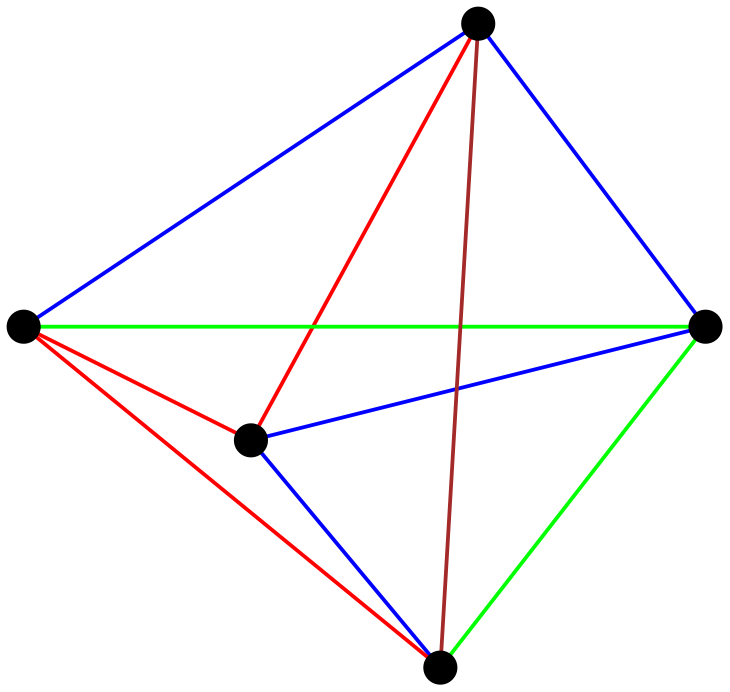
\includegraphics[width=0.4\linewidth]{images/decomposition_example}
\end{figure}
\end{frame}
\begin{frame}\frametitle{Thickness Geométrico}
	\begin{itemize}
		\item[] Entonces podemos definir el thickness $\theta(G)$ de una gráfica $G$ como el mínimo número de gráficas planares en una descomposición de $G$. 
		
		\item[] Y el thickness geométrico $\bar{\theta}(G)$ como el número mínimo de gráficas \emph{planas} que existen en una descomposición de $G$, para todos los \emph{dibujos geométricos} de $G$.
		
		\item[] En el año 2000, Dillencourt \emph{et al.} dan el valor exacto del \emph{thickness geométrico} para gráficas completas.\\[5pt]
	\end{itemize}
	
\end{frame}
\begin{frame}
	\begin{figure}
		\centering
		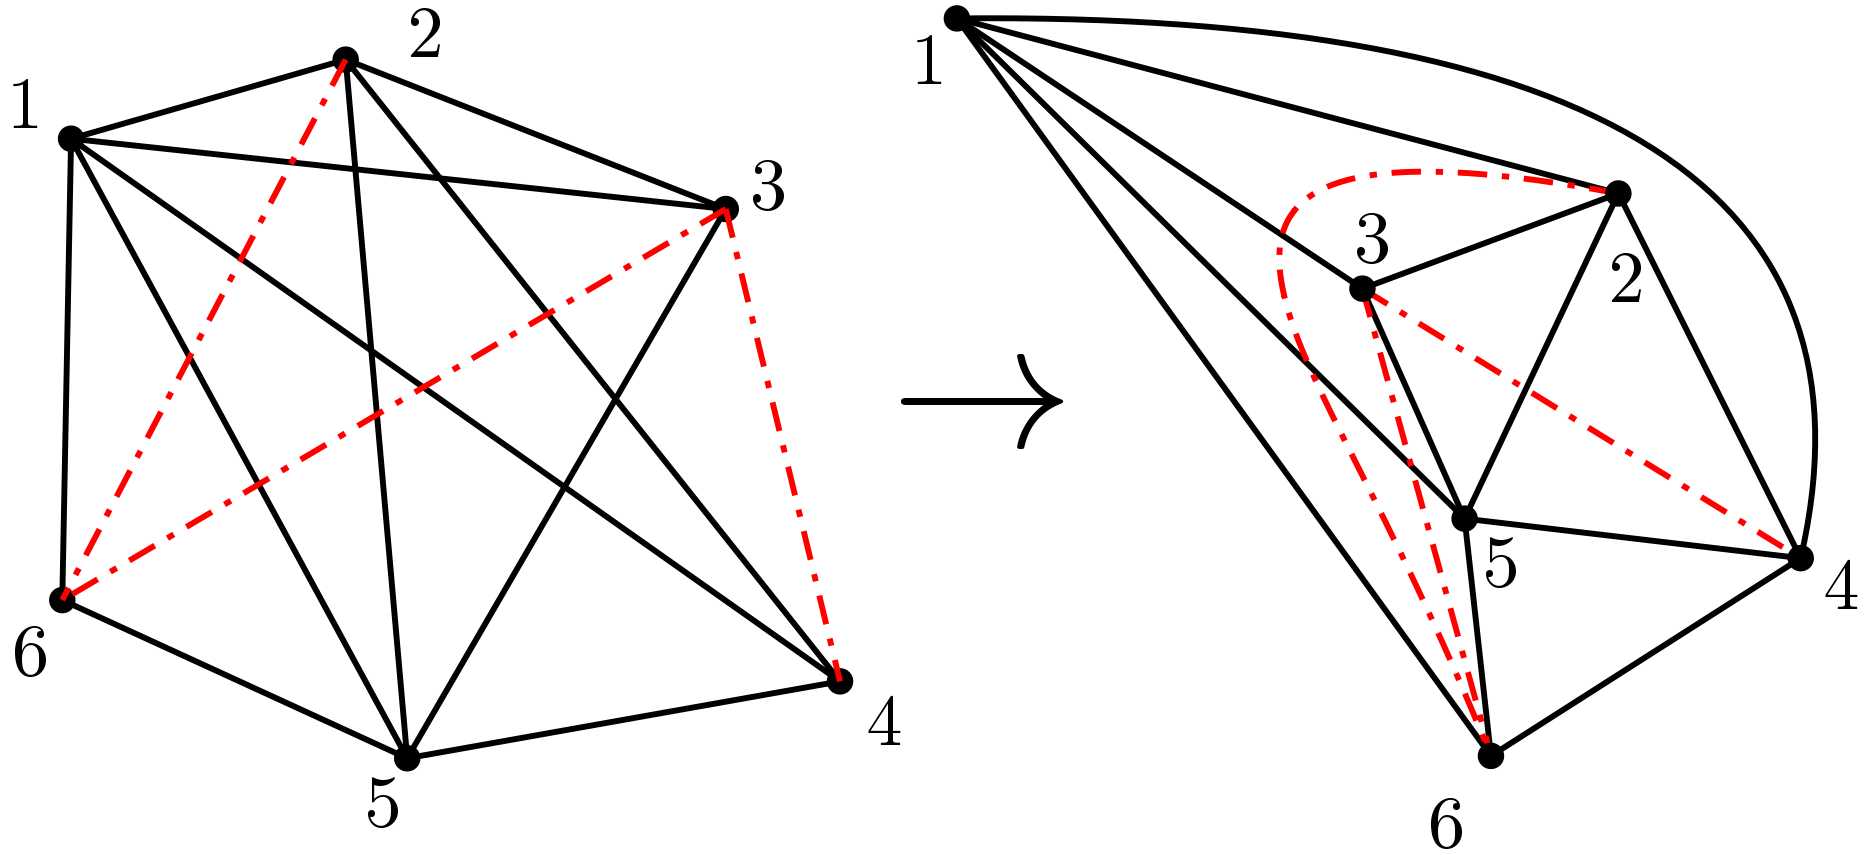
\includegraphics[width=0.6\textwidth]{images/K6_thicknes2}%
		~\vrule
		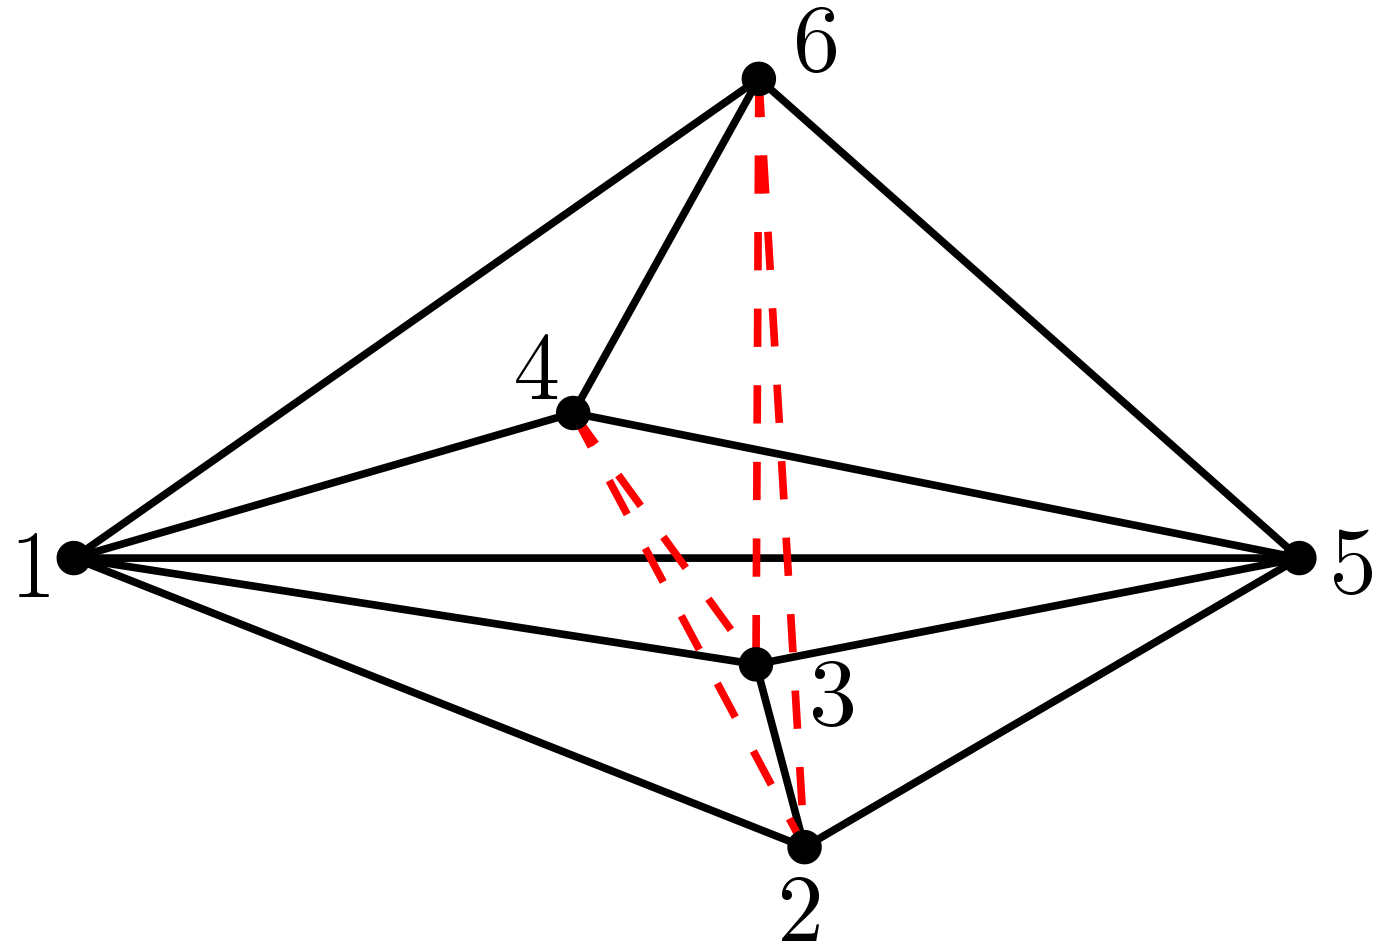
\includegraphics[width=0.4\textwidth]{images/K6_gthicknes2}
	\end{figure}
\end{frame}

\begin{frame}\frametitle{Gráfica de cruce}
Nosotros llamamos gráfica de cruce $E_{pp}(S)$ la gráfica cuyo conjunto de aristas es cada una de las aristas de $K_n(S)$ y cuyo conjunto de aristas contiene la información de los cruces de $K_n(S)$. Es decir, existe una arista entre dos vértices cuando sus aristas correspondientes en $K_n(S)$ se cruzan.
\end{frame}

\begin{frame}
\begin{figure}
	\centering
	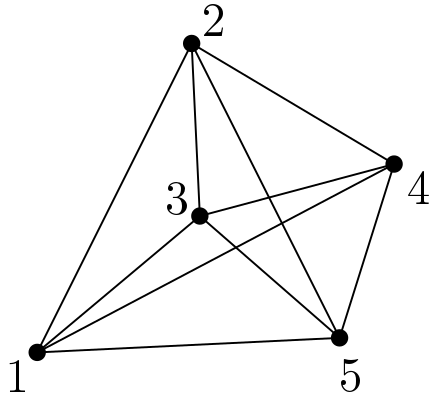
\includegraphics[width=0.26\textwidth]{images/K5}%
	~\vrule
	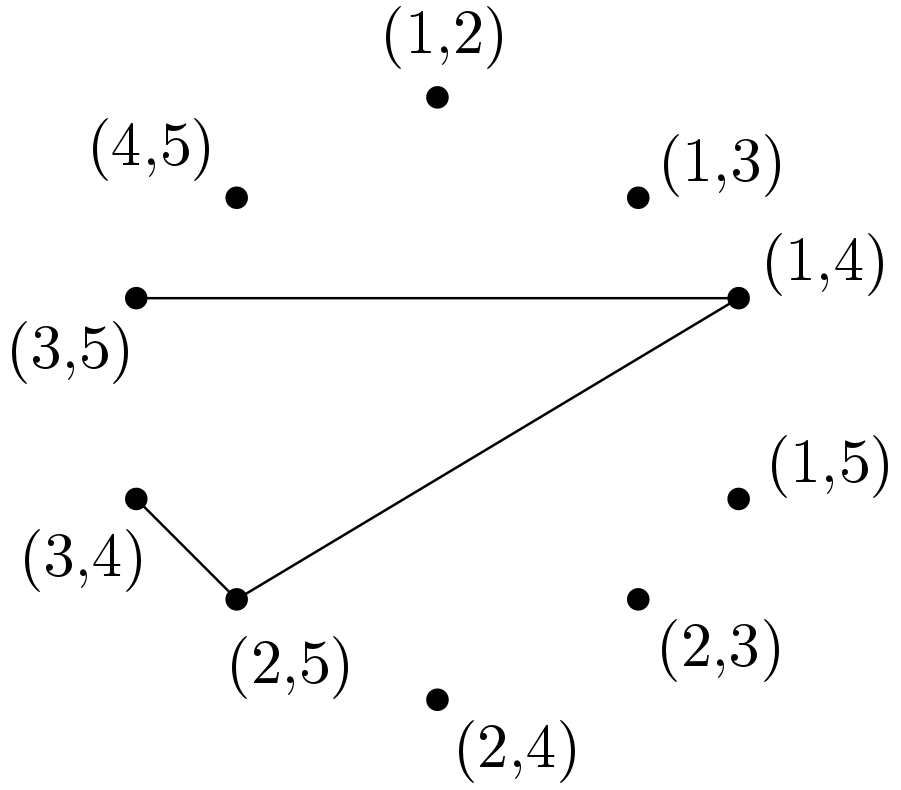
\includegraphics[width=0.35\textwidth]{images/EppK5}
	~\vrule
	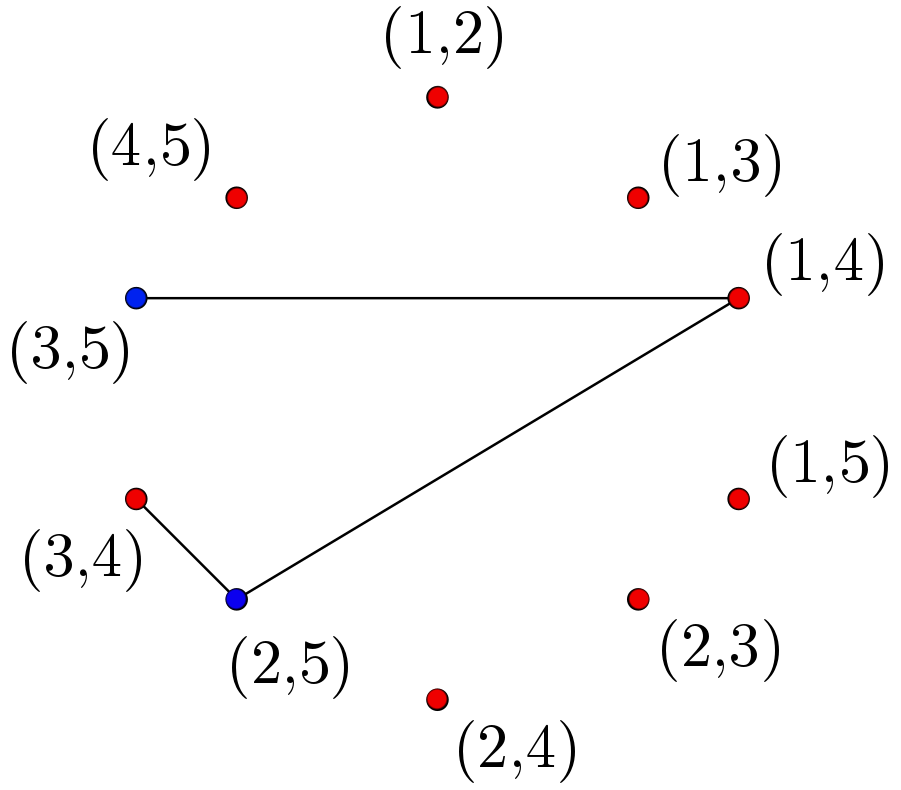
\includegraphics[width=0.35\textwidth]{images/EppK5_colored}
\end{figure}
Si encontramos una coloración propia de $C(S)$ las clases cromáticas representan gráficas planas. Luego, el número cromático $\chi(C(S))$\let\thefootnote\relax\footnote{El número cromático, $\chi(G)$, de $G$ es el mínimo número de clases cromáticas en una coloración propia de $G$.} nos dice el mínimo número de gráficas planas que hay en una descomposición de $K_n(S)$.

Por lo tanto: $\overline{\theta}(K_n(S)) = \min\{\chi(E_{pp}(S)) : S \subset \mathbb{R}^2, |S| = n\}$
\end{frame}

\begin{frame}\frametitle{Gráficas de adyacencia}
Es posible codificar la información de los cruces de las aristas de una gráfica geométrica usando un tipo de gráficas a las que llamamos \emph{gráficas de adyacencia}.

\begin{itemize}
	\item Las gráficas de adyacencia tienen como conjunto de vértices a las aristas de la gráfica completa que es inducida por algún conjunto $S$ de $n$ puntos.
\end{itemize}

	Existen otras gráficas de adyacencia a parte de $C(S)$, si consideramos otro criterio para definir las aristas de cada una podemos obtener diferentes resultados.
\end{frame}

\begin{frame}{Gráficas de adyacencia}
\begin{figure}
	\centering
	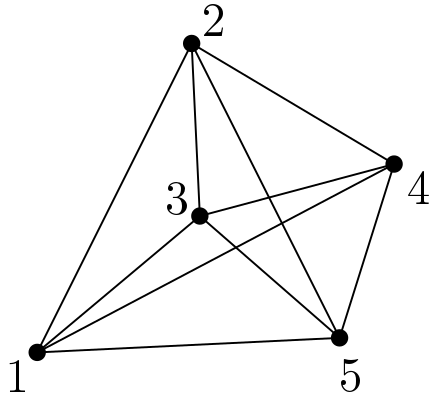
\includegraphics[width=0.3\textwidth]{images/K5}%
	~\vrule
	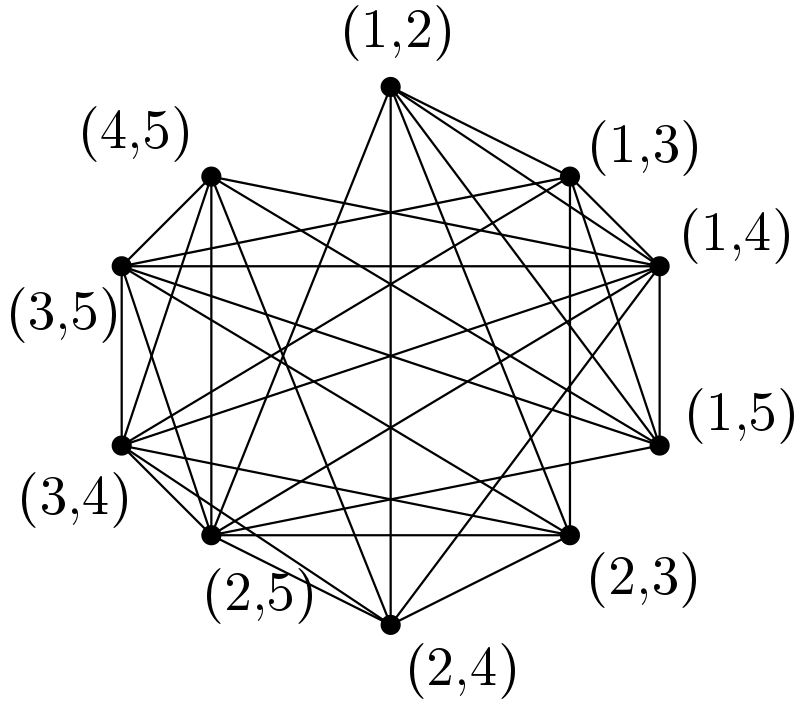
\includegraphics[width=0.35\textwidth]{images/grafica3k5}%
	~\vrule
	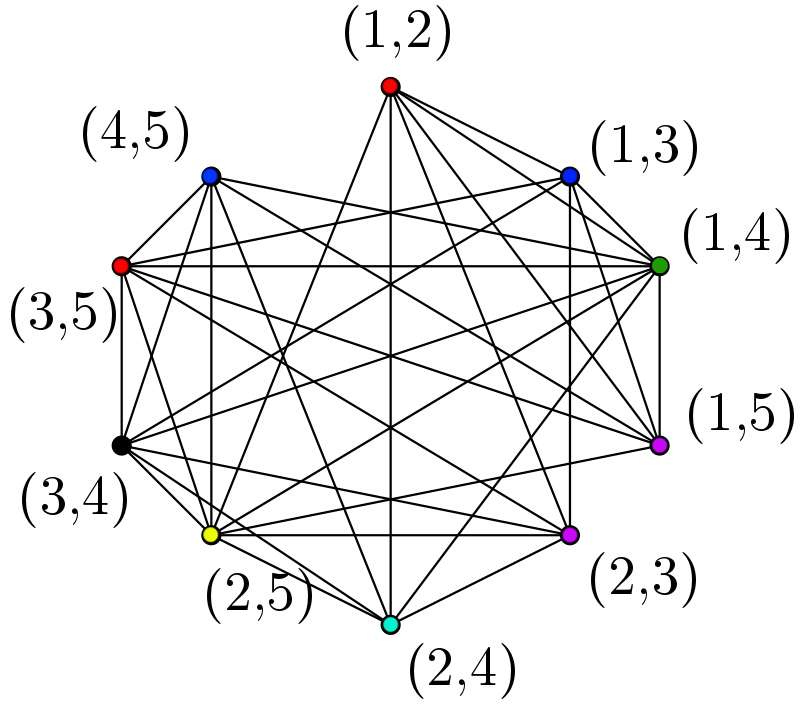
\includegraphics[width=0.35\textwidth]{images/grafica3k5_colored}%
\end{figure}

\begin{itemize}
\item $I(S)$: Existe una arista entre dos vértices si las aristas correspondientes comparten un vértice o se cruzan. Las clases cromáticas son \emph{emparejamientos planos}.

\end{itemize}
\end{frame}
\begin{frame}{Gráficas de adyacencia}
\begin{figure}
	\centering
	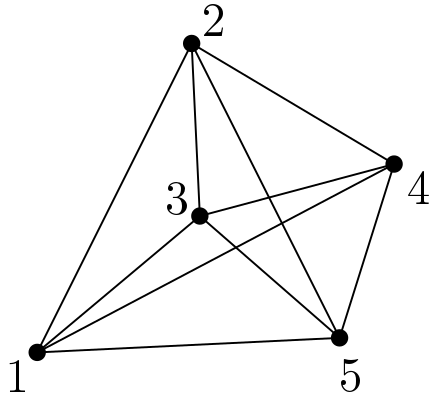
\includegraphics[width=0.3\textwidth]{images/K5}%
	~\vrule
	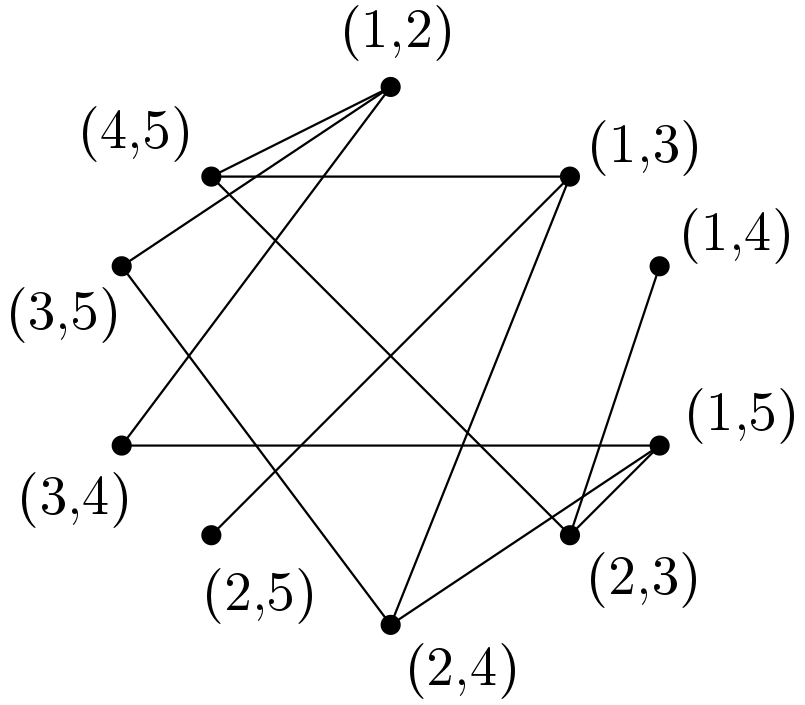
\includegraphics[width=0.35\textwidth]{images/grafica4k5}%
	~\vrule
	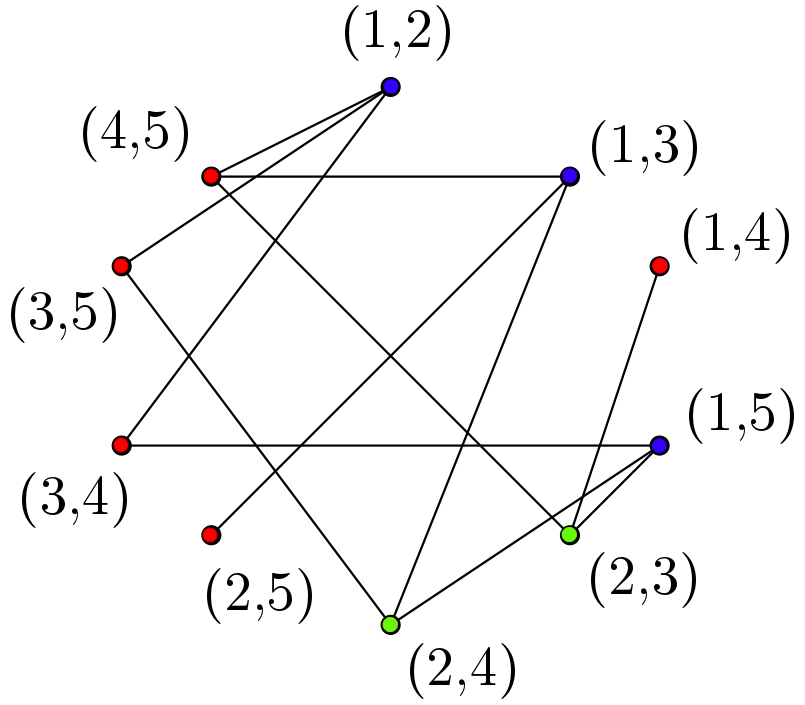
\includegraphics[width=0.35\textwidth]{images/grafica4k5_colored}%
\end{figure}

\begin{itemize}
\item $D(S)$: Existe una arista entre dos vértices si las aristas correspondientes son disjuntas. Las clases cromáticas son \emph{thrackles}.
\end{itemize}
\end{frame}

\setbeamercovered{invisible}
\begin{frame}{Descomposiciones de gráficas}
		En 2000, Dillencourt \emph{et al.} estudiaron: 
		\[ 
			\min\{ \chi(C(S)): S \subset \mathbb{R}^2,\text{ está en posición general}, |S|=n \}
		\]
		En 2005, Urrutia \emph{et al.} estudiaron: \[\max\{\chi(G(S)): S \subset \mathbb{R}^2 \text{ está en posición general, |S|=n} \}\] donde $G(S)$ es cada una de las gráficas $W(S),I(S),D(S)$. Ellos probaron cotas para estos parámetros. En otras palabras buscan el máximo número de crossing families, emparejamientos planos y thrackles necesarios en una descomposición de $K_n$.
\end{frame}
\begin{frame}{Descomposiciones de gráficas (Book thickness)}
	Una variante del problema del thickness se basa en colocar los puntos de la gráfica completa sobre un espacio geométrico diferente del plano, específicamente sobre una recta que es compartida por un número finito de semiplanos. 
	\begin{center}
		\only<1-3>{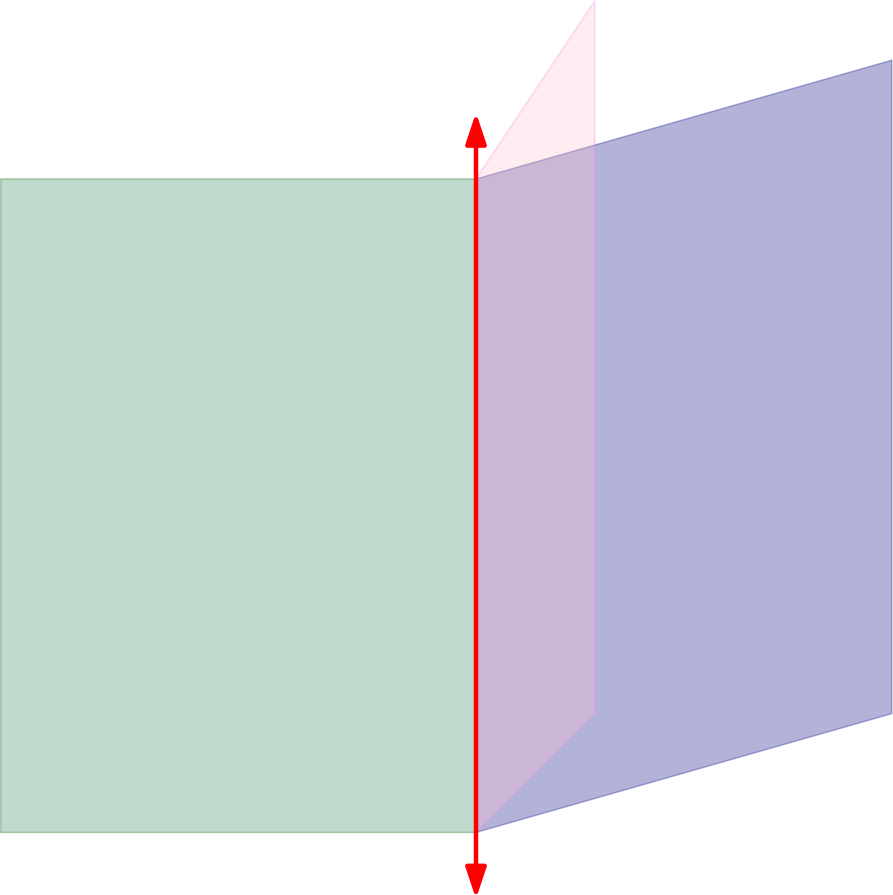
\includegraphics[width=0.4\linewidth]{images/book}}
		\only<2-3>{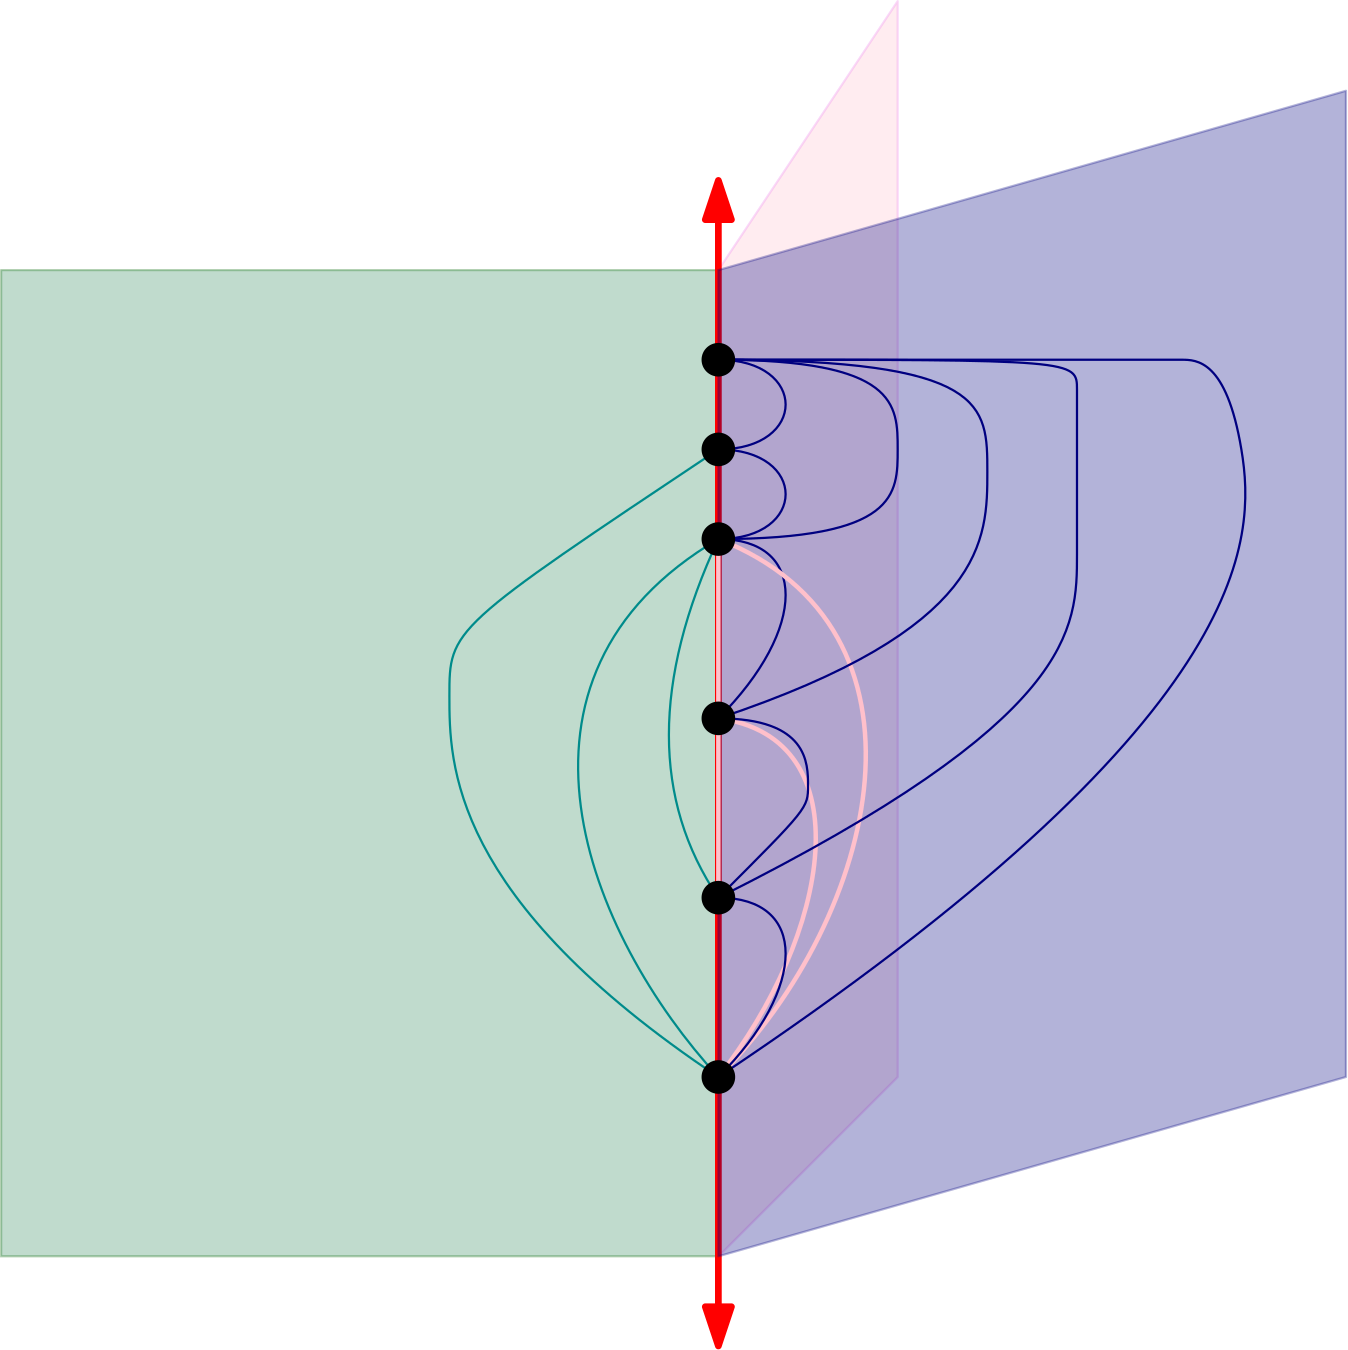
\includegraphics[width=0.4\linewidth]{images/book-thickness}}
	\end{center}
	\only<3>{
	\begin{itemize}
		\item El book-thickness es igual al thickness en posición convexa.
	\end{itemize}
	}	
\end{frame}
\begin{frame}
	\frametitle{Otras decomposiciones de gráficas}
	Solo en el plano:
	\begin{itemize}
		\item Bosques
		\begin{itemize}
			\item Star arboricity
			\item Linear arboricity
		\end{itemize}
		\item Hamiltoninan decomposition of complete graphs
		\item Cycle decomposition of complete graphs.
		\item \emph{Thrackles}
	\end{itemize}
	\begin{figure}
		\centering
		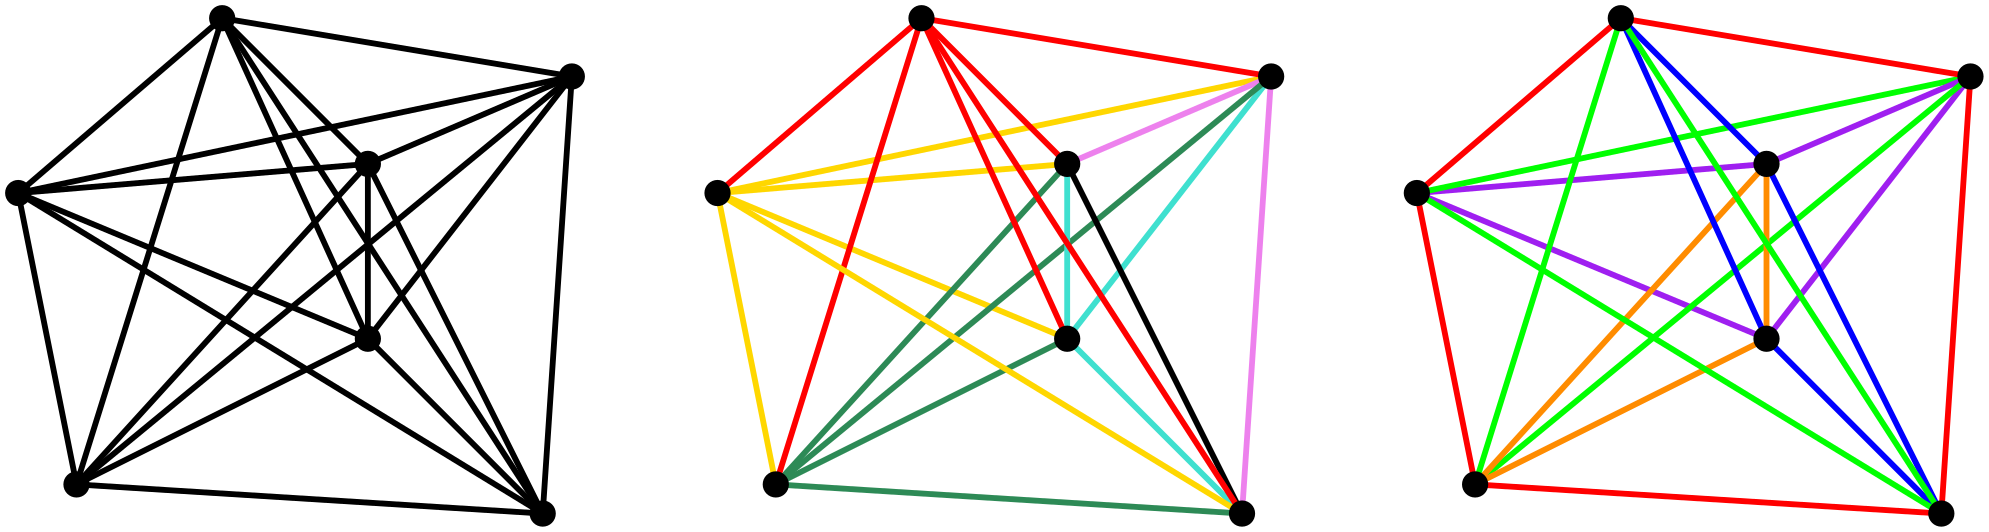
\includegraphics[width=1\linewidth]{images/other_decompositions}
	\end{figure}
\end{frame}

\begin{frame}{Anti-thickness geométrico}
\begin{figure}
	\centering
	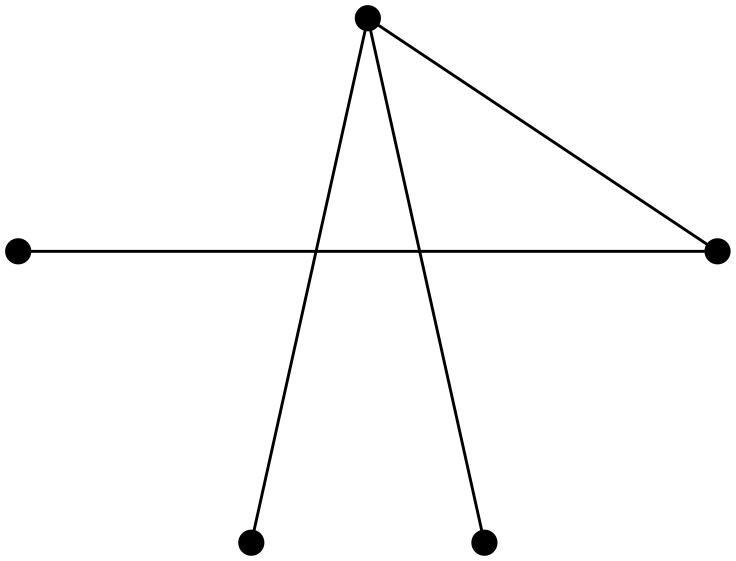
\includegraphics[width=0.35\linewidth]{images/thrackle_5}
	~\vrule~
	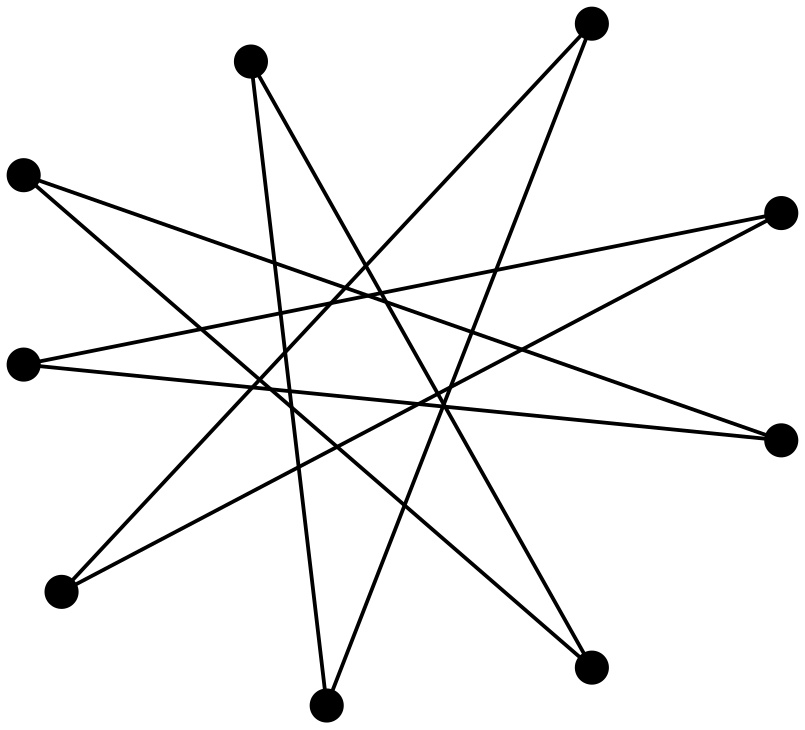
\includegraphics[width=0.3\linewidth]{images/thrackle_9}
\end{figure}
\begin{itemize}
	\item Un \emph{thrackle} es una gráfica geométrica en el que cada par de aristas se cruza o comparten un extremo.
	\item[] Sea $G$ una gráfica. El \emph{anti-thickness geométrico} mide cuántos thrackles geométricos existen, como mínimo y para todos los dibujos de $G$, en una descomposición por thrackles geométricos de $G$.
\end{itemize}

\end{frame}
\begin{frame}{Anti-thickness geométrico y el número cromático}
Recordemos que $\chi(D(S))$ nos indica cuántos thrackles geométricos hay en una descomposición de la gráfica completa inducida por $S$. 
\[
\min\{ \chi(D(S)) : S \subset \mathbb{R}^2\text{ está en posición general}, |S| = n \}
\] nos indica el mínimo numero de thrackles geométricos para todos los dibujos de alguna gráfica inducida por $S$, esto es, el anti-thickness geométrico.
\pause
\\[10pt]
Notación de anti-thickness geométrico de $K_n$: $At_g(K_n)$.

Observe que $At_g(K_n) = \min\{\chi(D(S)) \} = \max\{\chi(D(S)) \} = d(n)$ cuando $S$ es un conjunto de $n$ vértices en \emph{posición convexa}.
\end{frame}





% !TEX root=talk.tex
\section{Antecedentes}


\section{Resultados}
\begin{frame}
\frametitle{Anti-thickness geométrico}
Para $3 \leq n \leq 10$:
\[  At_g(K_n) = n - \left\lfloor\sqrt{2n + \frac{1}{4}} - \frac{1}{2} \right\rfloor \]
\end{frame}
\begin{frame}
\frametitle{Estado del arte}
Para $n \geq 3$:
\[  \frac{n-1}{2} \leq At_g(K_n) \leq n - \left\lfloor\sqrt{2n + \frac{1}{4}} - \frac{1}{2} \right\rfloor \]
Para encontrar alguna cota inferior es posible explotar alguna propiedad que se cumpla para todas las gráficas geométricas de $K_n$. Para encontrar una cota superior es posible ofrecer una descomposición de $K_n$ en thrackles.
\end{frame}
\begin{frame}
\frametitle{Estado del arte : cota inferior}
Erd\H{o}s \emph{et al.}(1988) probaron que cada gráfica geométrica con $n$ vértices en la cual no existen dos aristas disjuntas tiene a lo sumo $n$ aristas. 
\\[10pt]
Esto quiere decir que un thrackle máximo tiene a lo sumo $n$ aristas.
\end{frame}
\begin{frame}
\frametitle{Estado del arte : cota inferior}
En el trabajo de Wood \& Dujmovic se menciona que para $n \geq 3$:
\[  \frac{n-1}{2} \leq At_g(K_n).\] 
\pause

Esta cota inferior es la más sencilla, se basa en la noción del número máximo de aristas en un thrackle máximo. 
\\[5pt]
Si la gráfica completa tiene $\binom{n}{2} = \frac{n(n-1)}{2}$ aristas, ¿cuántos thrackles máximos son necesarios para \emph{cubrir} todas las aristas? Si suponemos que $k$ thrackles máximos\footnote{En el mejor caso, una descomposición por thrackles es inducida por una colección de thrackles máximos.} son necesarios la siguiente desigualdad nos otorga el resultado si resolvemos para $k$: \[ k\cdot n \geq \frac{n(n-1)}{2} \pause \Rightarrow k = \frac{n-1}{2}\]
\end{frame}

\begin{frame}
\frametitle{Estado del arte : cota superior}
Fabila-Monroy \emph{et al.} encuentran el anti-thickness exacto cuando $S$ está en posición convexa. Ellos estudian el problema del anti-thickness desde número cromático de $D(S)$. Para la cota inferior establecen el número mínimo de colores necesarios en una coloración propia de $D(S)$ y para la cota superior dan una coloración propia para cualquier $n$, con $n>3$.
\pause 
\\[10pt]
Ellos establecen que $\chi(D(S)) = n - \left\lfloor\sqrt{2n + \frac{1}{4}} - \frac{1}{2} \right\rfloor, $ cuando $S$ está en posición convexa.
\pause
\\[10pt]
Como la posición convexa es un dibujo de $K_n$ tenemos: \[At_g(K_n) \leq n - \left\lfloor\sqrt{2n + \frac{1}{4}} - \frac{1}{2} \right\rfloor. \]
\end{frame}
\begin{frame}
\frametitle{Estado del arte : thrackles máximos en posición convexa}
Un resultado del trabajo de Fabila-Monroy \emph{et al.} es que prueban que dos thrackles máximos en posición convexa siempre comparten al menos una arista. Esto significa que, en posición convexa y en el mejor caso, una colección de $k$ thrackles máximos cubre a lo sumo $kn - \binom{k}{2}$ aristas. Para obtener el valor más pequeño de $k$ podemos resolver, para $k$, la siguiente desigualdad :
\[
  kn - \binom{k}{2} \geq \binom{n}{2}.
\]
Usando la ecuación cuadrática encontramos que $k = n - \left\lfloor\sqrt{2n + \frac{1}{4}} - \frac{1}{2} \right\rfloor.$
\end{frame}
\begin{frame}
\begin{figure}
	\centering
	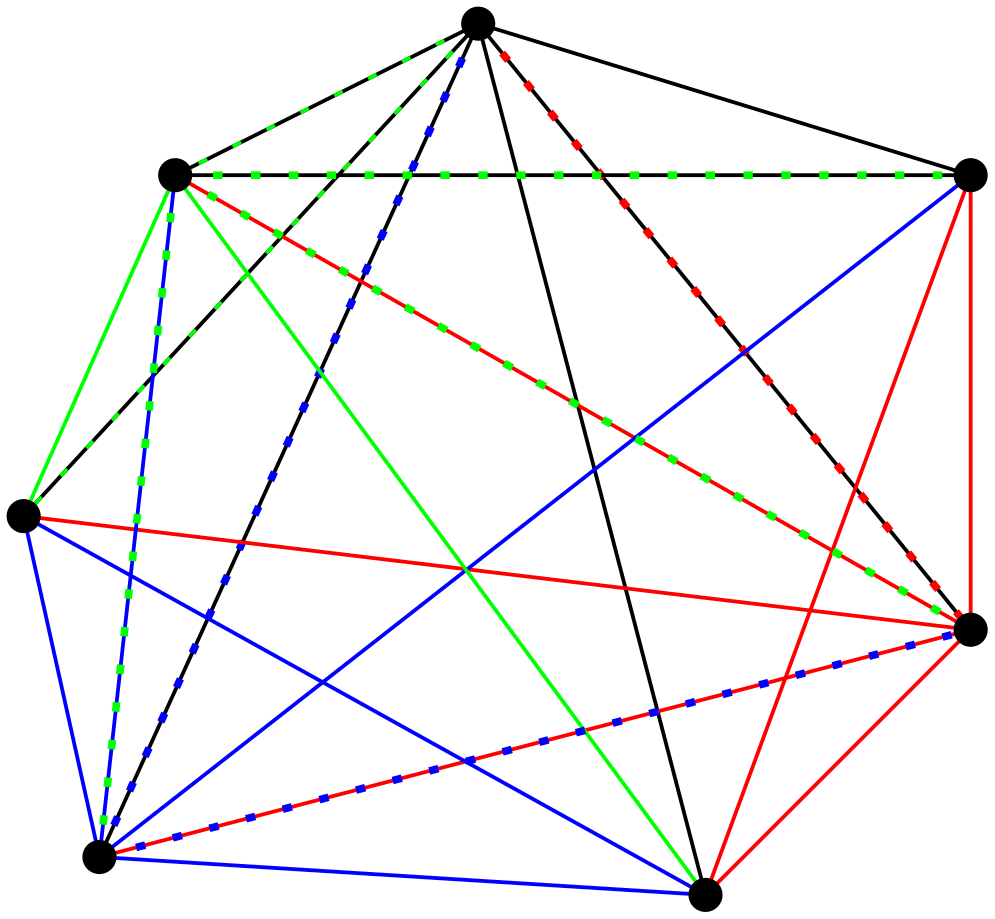
\includegraphics[width=0.75\linewidth]{images/thrackles_maximos}
\end{figure}
\end{frame}

\begin{frame}
\frametitle{Estado del arte : thrackles máximos en posición general}
\pause
\begin{itemize}
	\item En posición general es muy dificil dibujar thrackles máximos que sean disjuntos.
	\item La intuición nos dice que el resultado anterior es válido para posición general.
	\item ¿Cómo probamos \emph{todas} las gráficas geométricas de $K_n$?
\end{itemize}
\end{frame}

\begin{frame}
\frametitle{Tipo de orden}
Aichholzer \emph{et al.} definen el \emph{tipo de orden} de un conjunto $S=\{p_1,p_2,\dots p_n\}$ de puntos en posición general
como una función que asigna a cada tripleta ordenada $i,j,k\in\{1,2,\dots n\}$ la orientación de la tripleta de puntos $\{p_i,p_j,p_k\}$.
\begin{figure}
	\centering
	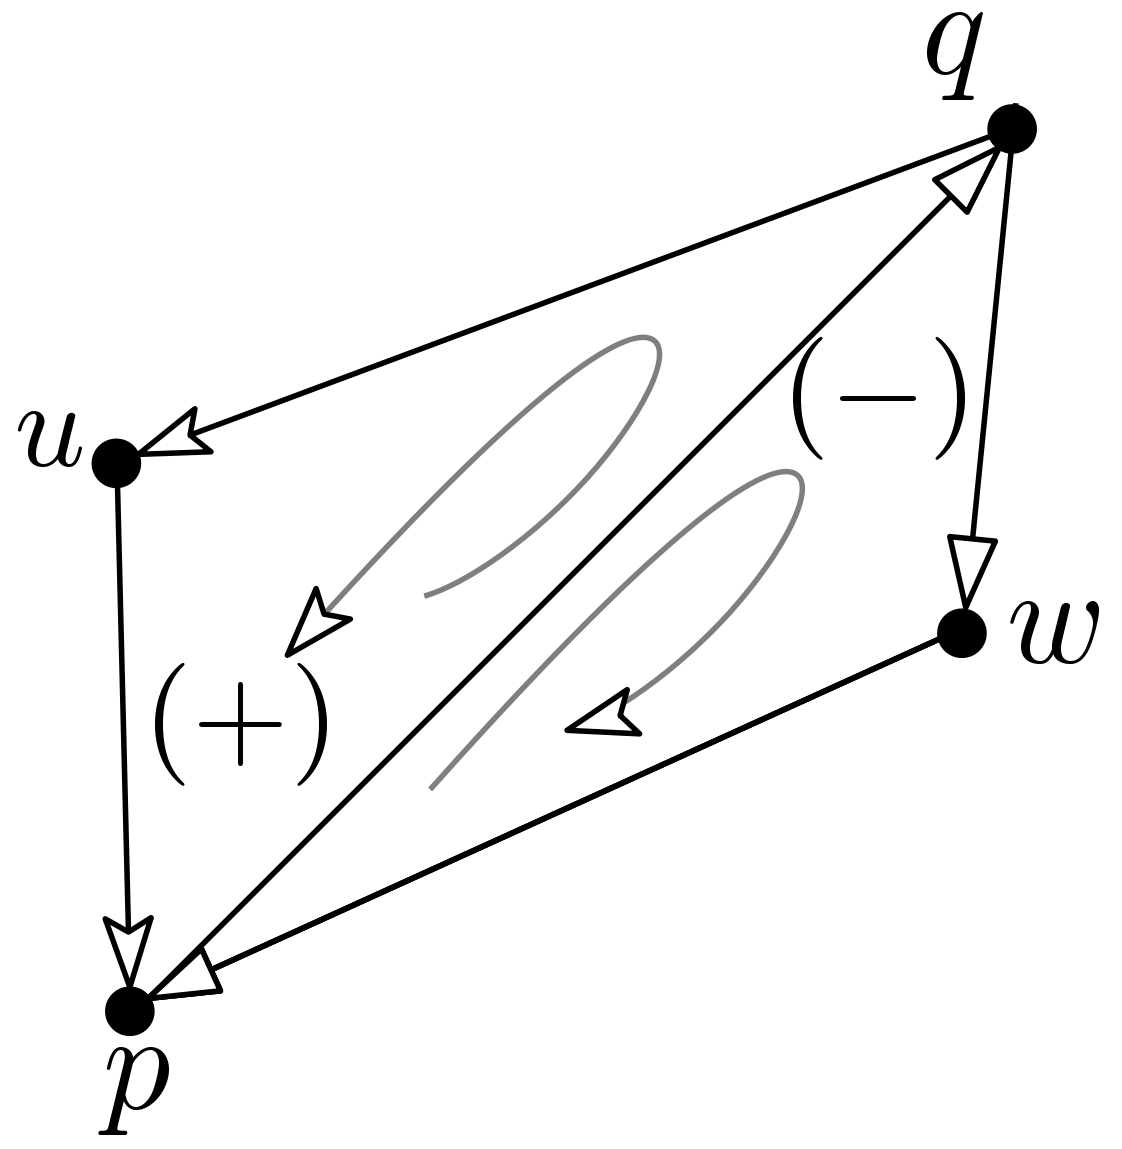
\includegraphics[width=0.3\linewidth]{images/triplet}
\end{figure}
Decimos que dos conjuntos de puntos $S_1$ y $S_2$ son combinatoriamente equivalentes cuando tienen el mismo tipo de orden.
\end{frame}

\begin{frame}
\frametitle{Tipo de orden}
Aichholzer \emph{et al.} ofrecen una base de datos para los tipos de orden de $3 \leq n \leq 10$.
\begin{table}[ht]
	\centering
	\begin{tabular}{|c|c|r|}
		\hline
		$n$ & Número de tipos de orden & Tamaño (bytes)   \\ \hline
		3     & 1                   & 6       \\ \hline
		4     & 2                   & 16      \\ \hline
		5     & 3                   & 30      \\ \hline
		6     & 16                  & 192     \\ \hline
		7     & 135                 & 1890    \\ \hline
		8     & 3315                & 53040   \\ \hline
		9     & 158817              & 5 717 412   \\\hline
		10    & 14309547            & 572 381 880 \\ \hline
	\end{tabular}
	\caption{Tipos de orden para cada $n\leq10$.}
	\label{tab:ots}
\end{table}
\end{frame}
\begin{frame}
\frametitle{Estado del arte : construyendo la nueva cota inferior}
Para analizar cada par de thrackles máximos en algun dibujo de $K_n$, primero hay que encontrarlos. Por ello, construimos un algoritmo 
exhaustivo que usa \emph{backtracking} para encontrar thrackles de cualquier tamaño. Nosotros llamamos $k-$thrackle a un thrackle de tamaño $k$.
Explicar algoritmo de búsqueda de $k$ thrackles y cómo hacemos la intersección.

\end{frame}

\begin{frame}
\frametitle{Estado del arte : construyendo la nueva cota inferior}
Una vez que hicimos las intersecciones de cada par de thrackles máximos en todos los dibujos de $K_n$, con $3 \leq n \leq 10$ encontramos los siguientes resultados:
\begin{itemize}
	\item Para todo tipo de orden con al menos dos thrackles máximos, cada par de thrackles máximos tienen intersección no vacía en aristas.
	\item Existen tipos de orden con solo un thrackle máximo.
	\item Existen tipos de orden en los que no hay thrackles máximos.
\end{itemize}
\end{frame}

\begin{frame}
\frametitle{Estado del arte : construyendo la nueva cota inferior}
Esto nos permite calcular el número exacto de aristas cubiertas, en el mejor caso, por una descomposición que es inducida por una colección de thrackles máximos. 

Nosotros probamos que, $m$ thrackles máximos pueden cubrir a lo sumo:
\[
-\frac{1}{2}m(m-2n-1)
\] aristas de la gráfica completa.
\pause 

\begin{table}
	\centering
\scalebox{0.7}{

	\begin{tabular}{	| >{\centering\arraybackslash}m{0.5in} | >{\centering\arraybackslash}m{0.8in} |  >{\centering\arraybackslash}m{1.2in} |  >{\centering\arraybackslash}m{1in} | }
		\hline
		$n$ & $m = \left\lceil\frac{n-1}{2}\right\rceil$ &     $-\frac{1}{2}m(m-2n-1) $ &
		$\binom{n}{2}$\\[5pt] \hline\hline
		3   & 1  & 3 & 3 \\ \hline
		4   & 2  & 7 & 6 \\ \hline
		5   & 2  & \cellcolor{red!25}9 & 10 \\ \hline
		6   & 3  & 15 & 15 \\ \hline
		7   & 3  & \cellcolor{red!25}18 & 21 \\ \hline
		8   & 4  & \cellcolor{red!25}26 & 28 \\ \hline
		9   & 4  & \cellcolor{red!25}30 & 36 \\ \hline
		10  & 5  & \cellcolor{red!25}40 & 45 \\ \hline
	\end{tabular}
}
\end{table}
\end{frame}

\begin{frame}
\frametitle{Estado del arte : construyendo la nueva cota inferior}
De la misma manera, para saber cuántos thrackles son necesarios para cubrir todas las aristas de la gráfica completa, debemos 
resolver la siguiente desigualdad para $m$:
\[
-\frac{1}{2}m(m-2n-1) \geq \binom{n}{2}.
\]
Usando la ecuación cuadrática encontramos que \[m =  n - \left\lfloor\sqrt{2n + \frac{1}{4}} - \frac{1}{2} \right\rfloor \]

\end{frame}
\begin{frame}
\frametitle{Estado del arte : construyendo la nueva cota inferior}
\begin{table}
	\centering
	\scalebox{0.9}{
		
		\begin{tabular}{	| >{\centering\arraybackslash}m{0.5in} | >{\centering\arraybackslash}m{1.6in} |  >{\centering\arraybackslash}m{1.2in} |  >{\centering\arraybackslash}m{1in} | }
			\hline
			$n$ & $m =  n - \left\lfloor\sqrt{2n + \frac{1}{4}} - \frac{1}{2} \right\rfloor $ &     $-\frac{1}{2}m(m-2n-1) $ &
			$\binom{n}{2}$\\[5pt] \hline\hline
			3   & 1  & 3 & 3 \\ \hline
			4   & 2  & 7 & 6 \\ \hline
			5   & 3  & 12 & 10 \\ \hline
			6   & 3  & 15 & 15 \\ \hline
			7   & 4  & 22 & 21 \\ \hline
			8   & 5  & 30 & 28 \\ \hline
			9   & 6  & 39 & 36 \\ \hline
			10  & 6  & 45 & 45 \\ \hline
		\end{tabular}
	}
\end{table}
Tenemos una nueva cota inferior para $3 \leq n \leq 10$:
\[ At_g(K_n) \geq n - \left\lfloor\sqrt{2n + \frac{1}{4}} - \frac{1}{2} \right\rfloor \] 
\end{frame}
\begin{frame}
\frametitle{Anti-thickness geométrico de $K_n$ para $3\leq n\leq 10$}
Con el resultado anterior y el resultado del estado del arte tenemos que, para $ 3 \leq n \leq 10$:
\[ n - \left\lfloor\sqrt{2n + \frac{1}{4}} - \frac{1}{2} \right\rfloor  \leq At_g(K_n) \leq n - \left\lfloor\sqrt{2n + \frac{1}{4}} - \frac{1}{2} \right\rfloor \] 
\pause
\[ At_g(K_n) = n - \left\lfloor\sqrt{2n + \frac{1}{4}} - \frac{1}{2} \right\rfloor \] 
\end{frame}

\begin{frame}
\frametitle{Anti-thickness geométrico de $K_n$ para $3\leq n\leq 10$}
\begin{itemize}
	\item[] Recordemos que la cota superior fue obtenida encontrando el anti-thickness de un dibujo específico, el que está en posición convexa.
	\item[] Recordemos que si $S$ es un conjunto de $n$ vértices en posición convexa, entonces \[ At_g(K(S)) = \min\{D(S)\} = \max\{D(S)\} = d(n)\]
\end{itemize}
¿Qué pasa con el anti-thickness de dibujos en posición general no convexa?
\end{frame}

\begin{frame}
\frametitle{Anti-thickness de dibujos en posición general no convexa}
\end{frame}
En esta tesis estudiamos el problema del anti-thickness geométrico de gráficas completas con hasta 10
vértices. El anti-thickness geométrico de una gráfica es el entero $k$ más pequeño tal que existe una
descomposición de la gráfica en $k$ thrackles. Un thrackle es una gráfica en la que cada par de aristas se
intersecta exactamente una vez.

En este trabajo encontramos que el anti-thickness geométrico $At_g(K_n)$ de la gráfica completa de $n$
vértices $K_n$, con $ 3 \leq n \leq 10$, es:
\[ At_g(K_n) =  n - \left\lfloor \sqrt{2n + \frac{1}{4}} - \frac{1}{2}\right\rfloor. \]
Para dar este resultado analizamos las gráficas completas inducidas por los conjuntos de hasta diez
vértices proveídos por la base de datos de tipos de orden del trabajo de~\cite{Aichholzer2001}, encontramos
que dos thrackles máximos de la misma gráfica completa comparten al menos una arista, dando así una nueva
cota inferior para conjuntos pequeños de puntos. La cota superior está dada por el anti-thickness del
dibujo de $K_n$ en posición convexa; nosotros encontramos dibujos, que no están en posición convexa, que
tienen el mismo anti-thickness.

Para cada thrackle de las descomposiciones encontradas calculamos el número
de cruce para observar que existe una relación del número de thrackles con número de cruce alto y número de
cruce bajo cercana al 50\%; en este trabajo damos la definición del número de cruce de un thrackle.

También analizamos y listamos cuáles conjuntos de puntos no tienen thrackles máximos y cuáles tienen
solamente un thrackle máximo para cada $n$ en el rango $[3,10]$. Aquí hacemos la observación de que
conjuntos con un número de cruce pequeño tienen menos thrackles máximos que los conjuntos con un número de
cruce elevado con respecto del número de cruce máximo para cada $n$ en el rango anteriormente mencionado.

Para los conjuntos de $n$ puntos, con $3 \leq n \leq 8$ que inducen gráficas completas sin thrackles
máximos analizamos, con un algoritmo exhaustivo, el anti-thickness geométrico de cada uno. Encontramos que
estos dibujos tienen anti-thickness mayor, en una unidad, al anti-thickness geométrico de $K_n$.

Uno de los objetivos de la tesis era obtener el anti-thickness geométrico de $K_n$ con $n\geq 3$. Sin
embargo no fue posible ya que no pudimos probar la generalización del lema~\ref{lema:thdisjuntos} que establece que la intersección entre dos thrackles máximos de un mismo dibujo siempre sucede. Decidimos no invertir más tiempo en la generalización del teorema para dar más resultados acerca de conjuntos pequeño de $n$.

\subsubsection{Trabajo futuro}

La generalización del lema~\ref{lema:thdisjuntos} es el trabajo a futuro más fuerte, de encontrarse, el
problema del anti-thickness geométrico para gráficas completas quedaría resuelto de manera general. Esto
deja abierto el problema de encontrar el anti-thickness de un dibujo en específico de manera eficiente.
Pero, como explicamos en el capítulo~\ref{cap3}, encontrar el anti-thickness de una gráfica geométrica
equivale a encontrar el número cromático de su gráfica de disyunción y este último es un problema
$NP$-difícil~(\cite{Skiena2003}). Sin embargo, existen algoritmos genéticos para encontrar una aproximación
al número cromático de una gráfica dada como los presentados en~\cite{Fleurent1996} y \cite{Galinier1999}
en los que se muestra que los resultados fueron obtenidos en un rango de tiempo considerablemente bueno
para el hardware en el que se implementaron. Es posible implementar estos algoritmos para encontrar la
coloración de la gráfica de disyunción y obtener resultados acerca del anti-thickness de algún dibujo de
$K_n$.

También es deseable encontrar una manera de caracterizar los dibujos que inducen gráficas completas sin
thrackles máximos, o con solo uno, ya que analizar todas las $\displaystyle \binom{\binom{n}{2}}{n}$
posibles combinaciones de $n$ aristas para buscar thrackles máximos puede resultar ineficiente,
especialmente con conjuntos grandes de puntos.

%\section{Wrapping Up} 
%
%\begin{frame}
%\frametitle{Summary}
%\begin{itemize}
%\item<+-> \hologo{LaTeX}
%	\begin {itemize}
%	\item a document preparation system
%	\item professional quality typesetting output
%	\end{itemize}
%\item<+-> Output artefacts
%	\begin{itemize}
%	\item Academic: papers, theses, books
%	\item Dedicated document types
%	\item Domain-specific material
%	\end{itemize}
%\item<+-> Usage scenario
%	\begin{itemize}
%	\item Direct authoring
%	\item Automatic generation (via scripts etc)
%	\item As back-end of other applications
%	\end{itemize}
%\end{itemize}
%\end{frame}
%
%\begin{frame}
%\centering
%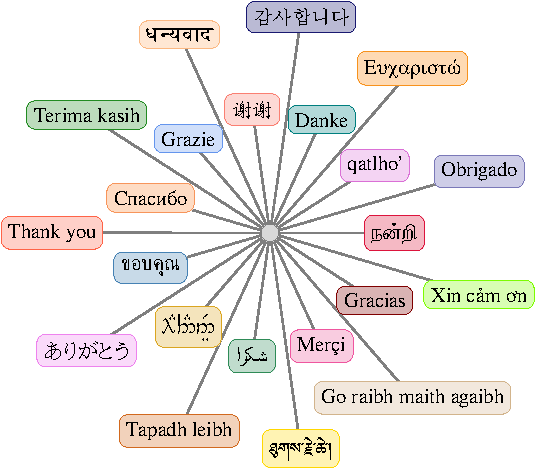
\includegraphics[width=.6\textwidth]{multiling-TQ}
%
%\bigskip 
%\begin{tabular}{cl}
%\multirow{2}{*}{\huge Questions?} & \url{liantze@gmail.com}, \url{support@overleaf.com}\\
%& \url{http://tex.stackexchange.com}\\
%\end{tabular}
%
%% {\huge Questions?\par}\vskip1em
%% {\large\url{liantze@gmail.com}
%% \\\url{support@overleaf.com}
%% \\\url{http://liantze.penguinattack.org}
%% \\\url{http://latex-my.blogspot.com}
%% \par}
%\end{frame}
%
%\begin{frame}
%\frametitle{Want to download this deck?}
%\centering
%\qrcode[height=.5\textheight]{https://www.overleaf.com/read/cyfvvyfrpmyn}
%\end{frame}
\begin{frame}%%     1
\begin{center}
	\Huge Thank You!
\end{center}
\end{frame}
\end{document}
